\subsection{Definition}
\begin{frame}
  \frametitle{Definition}
  \begin{block}{Zweck}
  	Kapselung eines Requests als Objekt, um so die Parametrisierung von Clients mit verschiedenen Requests, Warteschlangen- oder Logging-Operationen sowie das Rückgängigmachen von Operationen zu ermöglichen
  \end{block}
  
\end{frame}

\subsection{Klassendiagramm - Command Pattern}
\begin{frame}
	\frametitle{Observer Pattern}		
	\begin{itemize}
		\item Kapselt Request in ein eigenes Objekt Command
		\item Implementierung von Command kennt dann auch den Empfänger
	\end{itemize}	
  	\begin{figure}
		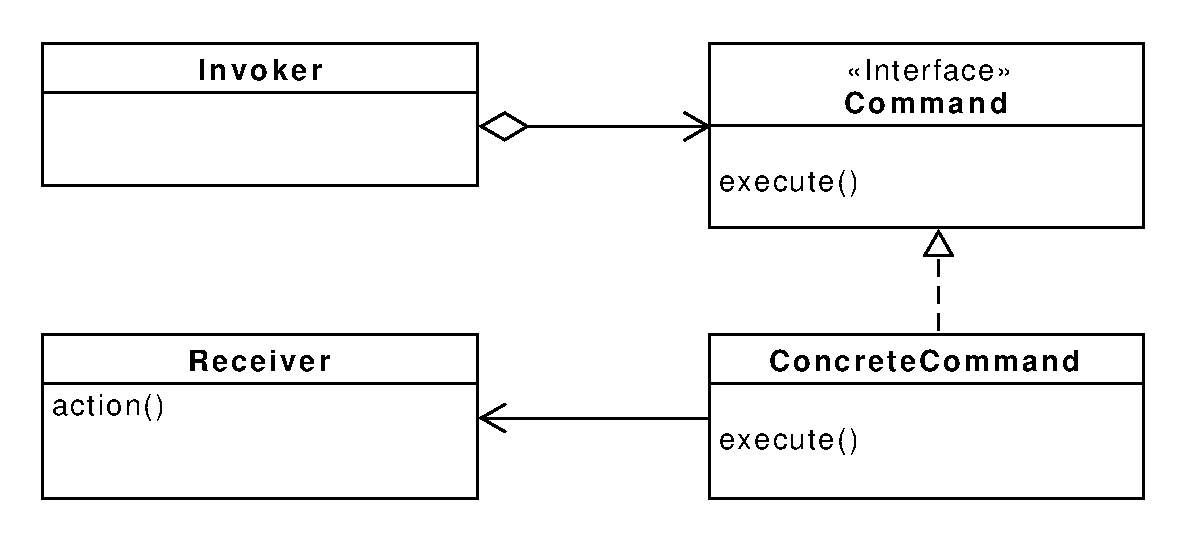
\includegraphics[scale=.4]{paper/command/command}
	\end{figure}
\end{frame}

\subsection{Beispiel - Deliver Service}
\begin{frame}
	\frametitle{Klassendiagramm}
	\begin{itemize}
		\item Verschiedene Objekte die unterschiedlich ausgeliefert werden müssen
		\item Unterschiedliche Kunden
	\end{itemize}	
	
  	\begin{figure}
		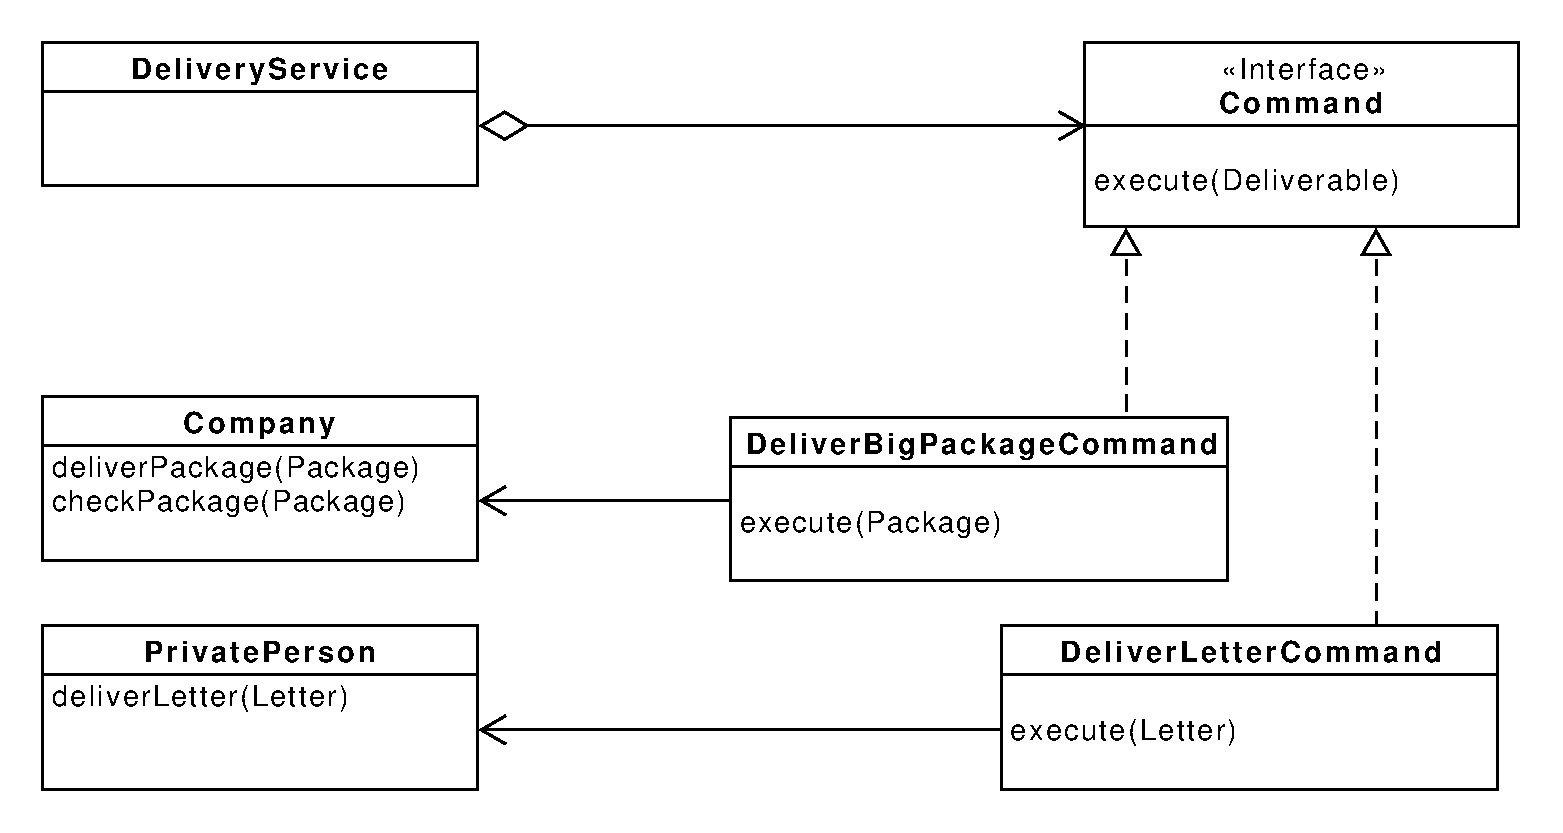
\includegraphics[scale=.4]{paper/command/DeliverService}
	\end{figure}
\end{frame}


\begin{frame}
	\frametitle{Command}
  	\begin{figure}
		\javacode{resources/command_interface.java} 
		\javacode{resources/command_DeliverBigPackageCommand.java} 
	\end{figure}
\end{frame}

\begin{frame}
	\frametitle{Command Interface}
  	\begin{figure}
		\javacode{resources/command_DeliveryService.java} 
		\javacode{resources/command_main.java}
	\end{figure}
\end{frame}

\subsection{Implementierung}

\begin{frame}
	\frametitle{Erweiterung}
  	\begin{block}{Undo-Funktion}
\begin{itemize}
		\item Erweiterung des Interfaces Command mit undo-Methode
		\item Der Invoker kann sich Commands merken und auf diese eine undo-Methode aufrufen
		\item das ConcreteCommand muss dann ggf. Daten speichern:
			\begin{itemize}
				\item Receiver-Objekt
				\item Die Argumente, die für die Ausführung angewendet wurden
				\item Alle relevanten Orginalwerte im Receiver-Objekt
			\end{itemize}
	\end{itemize}	
   \end{block}
\end{frame}

\begin{frame}
	\frametitle{Erweiterung}
  	\begin{block}{Makro-Befehle}
		\begin{itemize}
			\item Mehrere Receiver könnten gleichzeitig durch ein Command bearbeitet werden
		\end{itemize}	
   \end{block}
   \javacode{resources/command_macro_command.java}
\end{frame}



\begin{frame}
	\frametitle{Implementierungsmöglichkeit}
  	\begin{block}{Intelligenz der Commandobjekte}
		\begin{itemize}
		\item Command übernimmt vollständig die Logik
		\item Comnand delegiert die komplette Logik an den Receiver
	\end{itemize}	
   \end{block}
   
		\javacode{resources/command_command_logic.java}
\end{frame}


\subsection{Fazit}
\begin{frame}
	\frametitle{Fazit}
	\begin{columns} 
    	\column[t]{.50\textwidth} 
    		\begin{exampleblock}{Vorteile}
    			\begin{itemize}
    				\item Entkopplung von Befehl und Ausführung
    				\item Aufrufer können mit dem Interface Command arbeiten ohne wissen zu müssen, welche Operationen hinter den konkreten Commands stecken
    				\item Flexiblität indem Commands leicht ausgetauscht werden können
    			\end{itemize}
    		\end{exampleblock}
    	\column[t]{.50\textwidth} 
    		\begin{alertblock}{Nachteile}
    			\begin{itemize}
    				\item Hohe Anzahl von Klassen
    			\end{itemize}
    		\end{alertblock}
  	\end{columns}   	  		
\end{frame}